\section{Architektura VGG19}

Akronim VGG pochodzi od nazwy grupy badawczej \textit{Visual Geometry Group} z~uniwersytetu w~Oxfordzie będącej autorem analizowanej sieci. W~2014 roku zaproponowana przez naukowców z~\textit{VGG} architektura zdobyła pierwsze i~drugie miejsce kolejno w~kategorii lokalizacji i~klasyfikacji konkursu ImageNet \cite{vgg19}. Kluczową cechą ich modelu było zminimalizowanie wielkości filtrów warstw splotowych (a~co za tym idzie ilości związanych z~nimi parametrów) na rzecz zwiększenia ilości warst.

\vspace{0.5cm}
\begin{figure}[h]
    \centering
    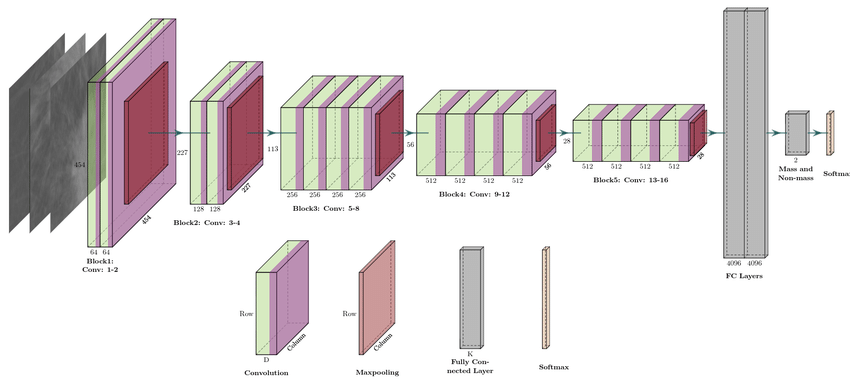
\includegraphics[scale=0.35]{img/vgg_structure.png}
    \label{vgg_structure_img}
    \caption{Struktura sieci VGG19}
\end{figure}
\vspace{0.5cm}

\noindent
VGG występuje w~kilku głównych wariantach oznaczanych przez VGG$x$, gdzie $x$ określa liczbę warstw sieci, których parametry są modyfikowanie w~czasie treningu. Rys. \ref{vgg_structure_img} prezentuje strukturę VGG19. Składa się ona z~trójwarstwowej części perceptronowej poprzedzonej kilkoma blokami konwolucyjnymi. W~skład każdego bloku wchodzi szereg warstw splotowych zakończony warstwą agregującą typu \textit{max pooling}. Rozmiar pola recepcyjnego wynosi odpowiedni $3\times3$ dla warstw splotowych i~$2\times2$ dla warstw agregujących. Warto w~tym miejscu zauważyć, że \textit{efektywne} pole recepcyjne dwóch połączonych warstw konwolucyjnych $3\times3$ ma wymiar $5\times5$ \cite{recept_field}. Podejście zaproponowane w~VGG ma jednak tę zaletę, że utylizuje większą ilość warstw nieliniowych, co według twórców przekłada się na ubogacenie fukncji decyzyjnej.

Ilość kanałów w~warstwach splotowych zwiększa się dwukrotnie w~każdym kolejnym bloku począwszy od 64 w~bloku wejściowym. Parametr \textit{stride} został ustalony na 1 w~warstwach splotowych oraz na 2 w~agregujących. Część perceptronowa składa się z~trzech warstw w~pełni połączonych o~odpowiednio 4096, 4096 i~1000 neuronach. W~warstwach ukrytych zastosowano nieliniowość typu \textit{ReLU}. Jedynie warstwa wyjściowa (klasyfikująca) wykorzystuje funkcję typu \textit{softmax}.